\documentclass[12pt]{article}
\title{Tripos Problem}
\author{By Katie James}

\usepackage{amsmath, amssymb, graphicx}
\usepackage{geometry}
\usepackage{titling}
\usepackage{tocloft}
\geometry{margin=1in}

%% \documentclass[tikz,border=10pt]{standalone}
\usepackage{amsmath}
\usepackage{tikz}
\usepackage{mathrsfs}
\usetikzlibrary{angles,quotes}



\usepackage{titling}
\renewcommand\maketitlehooka{\vspace*{5cm}}
\renewcommand\maketitlehookd{\vfill\null}

\date{}
\begin{document}

\begin{titlingpage}
\maketitle
\end{titlingpage}

\setlength{\parindent}{0pt}


\section*{Method 2 - Solving with Polar Coordinates}

\subsubsection*{Initial Impression}

Usually, to find the area under the curve, one would integrate $y dx$ where $y$ is defined as a function $f(x)$ of $x$. However, in this problem, both $x$ and $y$ are defined by the parameter $\theta$, which would naturally require parametric integration. I began by attempting the parametric method, however, I eventually found that the algebra involved was too intractable. I reasoned that there must be another method that would be less algebraically dense.

\vspace{\baselineskip}

An alternative way to perform the integral would be to integrate using polar coordinates. This requires us to transform the integration problem as stated from the Cartesian coordinates into polar coordinates.

\subsubsection*{Visualising the Polar Form}

I used the Pythagorean theorem and trigonometry to depict the transformation between Cartesian and polar coordinates.

\begin{figure}[h]
    \centering
    \includegraphics[width=0.5\linewidth]{polar graph.png}
    \caption{Cartesian to polar coordinate transformation.}
    \label{fig:figure1}
\end{figure}


%% \subsubsection*{What I already know}

By transforming the parametric equations defining the curve from $x$ and $y$ into the polar form:

\begin{align*}
    \hspace{1.25cm} x = \frac{\cos 3\theta}{\sin2\theta}  \hspace{1cm}  y = \frac{\sin 3\theta}{\sin2\theta}
\end{align*}

We can find the area in terms of the radius $r$ and polar angle $\phi$.

\begin{equation*}
    Area = \frac{1}{2} \int_{\phi_1}^{\phi_2}r^2 \, d\phi \\
\end{equation*}

\newpage

We begin by transforming $r$ using the Pythagorean definition of the radius

\begin{align*}
    r^2 &=x^2 + y^2  \\
    r^2 &= \frac{\cos^2 3\theta+sin^2 3\theta}{\sin^2 2\theta}  \\
\end{align*}

Using the identity $cos^2 3\theta+sin^2 3\theta=1$, the equation for $r^2$ can be further simplified

\begin{equation*}
    r^2 = \frac{1}{\sin^2 2\theta}.
\end{equation*}

We are now able to define the polar integral for the area as:

\begin{equation*}
    Area = \frac{1}{2} \int_{\phi_1}^{\phi_2}\frac{1} {\sin^2 2\theta} \, d\phi .  \\
\end{equation*}

The function we are integrating is defined in terms of $theta$. However, the integral is defined over infinitesimal changes of polar angle $\phi$ rather than in terms of changes over $\theta$. This is a problem that I had not previously encountered when integrating with polar coordinates. However, I figured that I could use my diagram in Figure \ref{fig:figure1} to find $d\phi$ in terms of $d\theta$.

\subsubsection*{Putting the Integral in Terms of $\theta$}

Using the trigonometric definition of $\tan \phi$ and definitions $x = r cos \phi$ and $y = r sin \phi$ from Figure \ref{fig:figure1} we find

\begin{align*}
\tan \phi = \frac{y}{x}
= \frac{\sin 3\theta \, \sin 2\theta}{\sin 2\theta \, \cos 3\theta}
= \frac{\sin 3\theta}{\cos 3\theta}
= \tan 3\theta
\end{align*}

\begin{equation*}
    \tan \phi = \tan 3\theta \qquad \Rightarrow \qquad \phi = 3\theta
\end{equation*}

Subsequently, we can differentiate the equation $\phi = 3\theta$

\begin{align*}
    \frac{d\phi}{d\theta} &= 3 \\
    \\
    d\phi &= 3\, d\theta
\end{align*}

and then substitute $d\phi$ into our integral for the area. We arrive at an equation for the area in terms of $\theta$.

\begin{equation*}
    Area = \frac12 \int_{\theta_1}^{\theta_2} r^2 \, 3\, d\theta
\end{equation*}

\begin{equation*}
    Area = \frac32 \int_{\theta_1}^{\theta_2} \frac{1}{\sin^2 2\theta}\, d\theta
\end{equation*}


\subsubsection*{Defining the Bounds of Integration}

A parametric plot of the function shows that function we wish to integrate is fully symmetric around both the $x$-axis and $y$-axis. Let us define the area in the first quadrant of the graph to be $A$ so that the total area is $Area = 4 A$.

\vspace{\baselineskip}

The first quadrant of the graph corresponds to the range of $\phi$ from $x=0$ to $y=0$. The corresponding values of the parameter $\theta$ can be found to be $\theta_1=\frac{\pi}{6}$ and $\theta_2=\frac{\pi}{3}$. We note that the same bounds can be used as when integrating using the parametric integration method, since the range of integration is in terms of $\theta$.

\vspace{\baselineskip}

Now we calculate the area  $A$ of the first quadrant

\vspace{\baselineskip}

\begin{equation*}
    A = \frac{3}{2} \int_{\pi/6}^{\pi/3} \frac{1}{\sin^{2}(2\theta)} \, d\theta.
\end{equation*}


\subsubsection*{Calculating the Integral}

Using simple integration, the rest of the problem can be routinely solved.

\begin{equation*}
    A = \frac{3}{2} \int_{\pi/6}^{\pi/3} \frac{1}{\sin^{2}(2\theta)} \, d\theta
\end{equation*}


\begin{equation*}
    A = \frac{3}{2} \left[ -\tfrac12 \cot(2\theta) \right]_{\pi/6}^{\pi/3}
\end{equation*}


\begin{equation*}
    A = \frac{3}{4} \left[ \left( -\frac{1}{\tan(\pi/3)} \right)
        - \left( -\frac{1}{\tan(\pi/6)} \right) \right]
\end{equation*}


\begin{align*}
    A &= \frac{3}{4} \left[ -\frac{\sqrt{3}}{3} + \sqrt{3} \right] \\
    A &= \frac{\sqrt{3}}{2}
\end{align*}

In conclusion, we are able to prove that the area enclosed by the parametric function is

\begin{equation*}
    Area = 4 A = 2\sqrt{3}
\end{equation*}

\newpage

\subsubsection*{\LaTeX  \hspace{0cm} Diagram}

\begin{figure}[h]
\centering
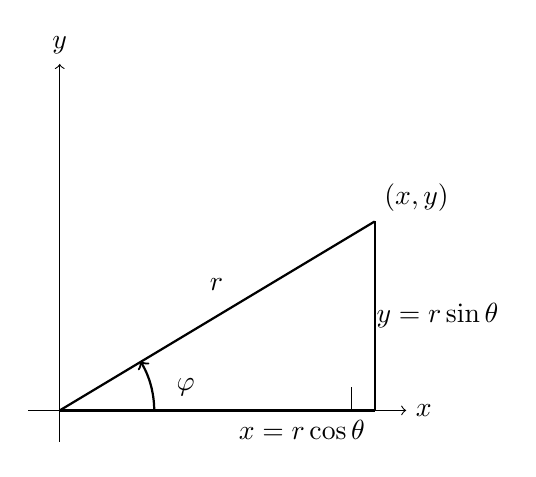
\begin{tikzpicture}[scale=2]
  % Axes
  \draw[->] (-0.2,0) -- (2.2,0) node[right] {$x$};
  \draw[->] (0,-0.2) -- (0,2.2) node[above] {$y$};

  % Point and triangle
  \coordinate (O) at (0,0);
  \coordinate (P) at (2,1.2);
  \draw[thick] (O) -- (P);
  \draw[thick] (P) -- (2,0);
  \draw[thick] (O) -- (2,0);

  % Labels
  \node[above right] at (P) {$(x, y)$};
  \node[below left] at (2,0) {$x = r\cos\theta$};
  \node[right] at (1.95,0.6) {$y = r\sin\theta$};
  \node[above left] at (1.1,0.7) {$r$};

  % Angle
  \draw[->, thick] (0.6,0) arc[start angle=0,end angle=31.5,radius=0.6];
  \node at (0.8,0.15) {$\varphi$};

  % Right angle marker
  \draw (2,0) -- ++(-0.15,0) -- ++(0,0.15);

\end{tikzpicture}
\caption{Polar to Cartesian coordinate conversion}
\end{figure}


\end{document}
